\chapter{Mul-Variational Auto-Encoder}
\ifpdf
    \graphicspath{{Chapter3/Chapter3Figs/PNG/}{Chapter3/Chapter3Figs/PDF/}{Chapter3/Chapter3Figs/}}
\else
    \graphicspath{{Chapter3/Chapter3Figs/EPS/}{Chapter3/Chapter3Figs/}}
\fi
\label{chap_3}
\begin{quote}
\textit{Chương này trình bày về những đóng góp của luận văn. Ở đây, Chúng tôi phân tích hai loại dữ liệu phản hồi chính từ người dùng là :"explicit feedback" và "implicit feedback". Đặc biệt, chúng tôi tập trung nghiên cứu mở rộng mô hình ``Variational Auto-Encoders'' cho implicit feedback với hàm lỗi là ``Multinomial Log-likelihood'' ở hàm mục tiêu. Chúng tôi gọi ``Variational Auto-Encoders''  với hàm lỗi như vậy là ``Mul-VAE''. Đóng góp của chúng tôi là làm rõ Mul-VAE ở hai điểm:
\begin{itemize}
	\item Tính xếp hạng: Chúng tôi chỉ ra điểm phù hợp của Multinomial Log-likelihood cho bài toán xây dựng hệ thống gợi ý sản phẩm so với các hàm Log-likelihood thông dụng khác.
	\item KL-Annealing: chúng tôi cũng đưa ra một cách "heuristic" nhằm lựa chọn siêu tham số của mô hình Mul-VAEs.
\end{itemize}}
\end{quote}

\section{"Explicit Feedback" và "Implicit Feedback"}
Các hàm kích hoạt thường được sử dụng trong mạng nơ-ron là:
\begin{itemize}
\item hàm sigmoid: $f(x) = \frac{1}{1+e^{-x}}$ 
\item và hàm tanh: $f(x) = \frac{e^x - e^{-x}}{e^x + e^{-x}}$
\end{itemize}
Gần đây, cộng đồng nghiên cứu mạng nơ-ron phát hiện ra một hàm kích hoạt mới hoạt động rất tốt là hàm ``rectified linear'' \cite{nair2010rectified}\cite{glorot2011deep}\cite{zeiler2013rectified}: $f(x) = max(0, x)$.

Hàm kích hoạt ``rectified linear'' rất phù hợp với ``Sparse Auto-Encoders''  (SAEs) bởi vì hàm này vốn dĩ đã tạo ra véc-tơ đặc trưng thưa (với một véc-tơ đầu vào, hàm ``rectified linear'' vốn dĩ đã tạo ra một véc-tơ đặc trưng với khoảng 50\% số phần tử bằng 0). Khác với hàm sigmoid là khi véc-tơ đầu vào không chứa đặc trưng tương tự với đặc trưng của bộ lọc (ở đây bộ lọc ám chỉ véc-tơ gồm các trọng số đi vào một nơ-ron ẩn), hàm ``rectified linear'' thường sẽ cho giá trị đúng bằng 0; trong khi đó, hàm sigmoid thường vẫn cho một giá trị dương nhỏ. Ngoài ra, hàm ``rectified linear'' tính nhanh hơn hàm sigmoid và hàm tanh bởi vì hàm này chỉ phải thực hiện phép max chứ không phải thực hiện phép lũy thừa và phép chia như ở hai hàm kia. Cuối cùng, hàm ``rectified linear'' có tiềm năng để có thể huấn luyện đồng thời nhiều tầng biểu diễn đặc trưng một cách không giám sát (thay vì phải huấn luyện từng tầng biễu diễn đặc trưng một) bởi vì hàm này đã được dùng để huấn luyện thành công nhiều tầng biểu diễn đặc trưng trong ngữ cảnh có giám sát \cite{glorot2011deep}\cite{zeiler2013rectified}. Với những điểm trên, trong luận văn này, chúng tôi sẽ tập trung nghiên cứu SAEs với hàm kích hoạt ở tầng ẩn là hàm ``rectified linear''. Chúng tôi gọi SAEs với hàm kích hoạt như vậy là ``Sparse Rectified Auto-Encoders''  (SRAEs).
\section{"Mul-VAEs" - Mở rộng VAE cho bài toán gợi ý sản phẩm}

Cách thường được dùng để ràng buộc thưa trong ``Sparse Auto-Encoders''  (SAEs) là ép giá trị đầu ra trung bình $\bar{h}_j$ của nơ-ron ẩn thứ $j$ về một giá trị cố định gần không $\rho$ \cite{goodfellow2009measuring}\cite{coates2011analysis}\cite{coates2012demystifying} (giá trị đầu ra trung bình này được tính với toàn bộ các mẫu huấn luyện, hoặc nếu dùng ``mini-batch'' thì sẽ được tính với các mẫu huấn luyện trong một ``mini-batch'' nhưng kích thước của ``mini-batch'' cần phải tương đối lớn). Trong trường hợp giá trị đầu ra của nơ-ron ẩn thuộc $[0, 1]$ (ví dụ, dùng hàm kích hoạt sigmoid), việc ép thưa có thể được thực hiện bằng cách cực tiểu hóa sự sai biệt Kullback-Leibler (KL):
\begin{equation}
	\sum_jKL(\rho||\bar{h}_j) = \sum_j\left(\rho\log\frac{\rho}{\bar{h}_j} + (1-\rho)\log\frac{(1-\rho)}{(1-\bar{h}_j)}\right)
	\label{eq_lifetime_KL}
\end{equation}
Khi $\bar{h}_j$ càng gần với $\rho$ thì hàm $KL(\rho||\bar{h}_j)$ sẽ có giá trị càng nhỏ và sẽ đạt cực tiểu (bằng $0$) khi $\bar{h}_j = \rho$; khi $\bar{h}_j$ càng xa với $\rho$ ($\bar{h}_j$ tiến về phía $0$ hoặc phía $1$) thì hàm $KL(\rho||\bar{h}_j)$ sẽ có giá trị càng lớn và tiến tới $\infty$ khi $\bar{h}_j$ tiến tới $0$ hoặc tiến tới $1$ (minh họa ở hình \ref{fig_KL}). Trong trường hợp dùng hàm kích hoạt ``rectified linear'', ta có thể dùng độ lỗi bình phương để ép $\bar{h}_j$ về $\rho$:
\begin{equation}
	\sum_j(\bar{h}_j - \rho)^2
	\label{eq_lifetime_SE}
\end{equation}

\begin{figure}
	\centering
	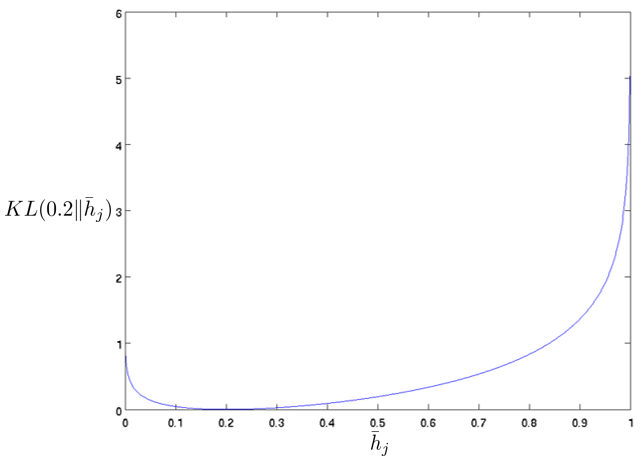
\includegraphics[width=0.8\textwidth]{KL}
	\caption[Minh họa hàm $KL(\rho\|\bar{h}_j)$ với $\rho=0.2$]{Minh họa hàm $KL(\rho\|\bar{h}_j)$ với $\rho=0.2$. Khi giá trị đầu ra trung bình $\bar{h}_j$ của nơ-ron ẩn $j$ càng gần $\rho$ thì $KL(\rho\|\bar{h}_j)$ sẽ có giá trị càng nhỏ và $KL(\rho\|\bar{h}_j)$ sẽ đạt cực tiểu (bằng $0$) khi $\bar{h}_j = \rho$; khi $\bar{h}_j$ càng xa với $\rho$ ($\bar{h}_j$ tiến về phía $0$ hoặc phía $1$) thì hàm $KL(\rho||\bar{h}_j)$ sẽ có giá trị càng lớn và tiến tới $\infty$ khi $\bar{h}_j$ tiến tới $0$ hoặc tiến tới $1$.}
	\label{fig_KL}
\end{figure}

Lưu ý là cách ràng buộc thưa này (ép các giá trị đầu ra trung bình của các nơ-ron ẩn về một giá trị cố định gần không) không trực tiếp làm thưa véc-tơ đặc trưng (véc-tơ gồm các giá trị đầu ra ở tầng ẩn khi đưa vào SAEs một véc-tơ đầu vào), mà làm thưa véc-tơ chứa các giá trị của một đặc trưng (véc-tơ gồm các giá trị đầu ra của một nơ-ron ẩn khi đưa vào SAEs các véc-tơ đầu vào khác nhau). Tuy nhiên, cách ràng buộc này làm thưa véc-tơ đặc trưng một cách gián tiếp. Để hình dung rõ hơn về điểm này, ta xét một ví dụ đơn giản sau. Giả sử tập huấn luyện của ta gồm có 5 mẫu huấn luyện và SAEs của ta gồm có 3 nơ-ron ẩn (ứng với 3 đặc trưng). Như vậy ta sẽ có ma trận đặc trưng có kích thước $3\times 5$, trong đó mỗi cột là một véc-tơ đặc trưng ứng với một mẫu huấn luyện (một véc-tơ đầu vào), mỗi dòng là một véc-tơ gồm 5 giá trị của một đặc trưng ứng với 5 mẫu huấn luyện. Cách ràng buộc thưa ở trên sẽ làm thưa các véc-tơ dòng của ma trận này; giả sử mỗi véc-tơ dòng này chỉ có một phần tử khác không và bốn phần tử còn lại bằng không. Bởi vì từ mỗi véc-tơ cột ta cần phải tái tạo lại véc-tơ đầu vào tương ứng, nên ta cần phân bố các phân tử khác 0 trải đều trên toàn các véc-tơ cột, cố gắng sao cho mỗi véc-tơ cột đều có phần tử khác 0 (nếu ta tập trung các phần tử khác 0 trên cùng một véc-tơ cột thì chỉ có một véc-tơ đầu vào tương ứng được tái tạo tốt, các véc-tơ đầu vào còn lại sẽ không được tái tạo tốt). Và điều này dẫn đến các véc-tơ cột cũng sẽ thưa.

Tuy nhiên, cách ràng buộc thưa như trên đưa thêm một siêu tham số (giá trị đầu ra trung bình mong muốn $\rho$) vào danh sách các siêu tham số vốn đã có rất nhiều của SAEs (hệ số ``thỏa hiệp'' giữa độ lỗi tái tạo và độ thưa, số lượng node ẩn, hệ số học, kích thước ``mini-batch'', ...). Điều này sẽ làm cho quá trình chọn lựa các siêu tham số trở nên ``phiền phức'' hơn và tốn thời gian hơn. 

Tại sao lại không dùng chuẩn L1 để ràng buộc thưa trong SAEs? Đây là một cách tự nhiên vì chuẩn L1 đã được dùng để ràng buộc thưa trong Sparse Coding. Hơn nữa, chuẩn L1 không đưa thêm siêu tham số nào. Ngoài ra, cách tính chuẩn L1 cũng rất đơn giản; trong trường hợp dùng hàm kích hoạt ``rectified linear'', chuẩn L1 của véc-tơ đặc trưng $h$ đơn giản là bằng tổng giá trị các phần tử của $h$. Trong phần dưới đây, chúng tôi sẽ giải thích về khó khăn gặp phải khi huấn luyện SAEs, cụ thể là SRAEs, với chuẩn L1.
\subsection{Huấn luyện mô hình}
Vấn đề gặp phải khi huấn luyện SRAEs với chuẩn L1 là trong quá trình tối ưu hóa hàm chi phí, chuẩn L1 có thể đẩy véc-tơ gồm các trọng số đi vào một nơ-ron ẩn vào trạng thái mà ở đó nơ-ron ẩn luôn luôn không kích hoạt (có giá trị đầu ra bằng 0 với tất cả các mẫu trong tập huấn luyện). Và một khi véc-tơ trọng số đi vào này đã rơi vào trạng thái nói trên, nó sẽ bị mắc kẹt ở đó mãi mãi và không bao giờ được cập nhật nữa; véc-tơ trọng số đi ra của nơ-ron ẩn này cũng không bao giờ được cập nhật nữa. Một cách cụ thể, xét một nơ-ron ẩn $j$: có trọng số $W^{(e)}_{ji}$ nối với nơ-ron đầu vào $i$, và có trọng số $W^{(d)}_{kj}$ nối với nơ-ron đầu ra $k$. Các đạo hàm riêng của hàm chi phí $C$ (hàm chi phí của một mẫu huấn luyện) ở công thức (\ref{eq_SAE}) (với hàm ép thưa $s(\cdot)=||\cdot||_1$) theo $W^{(e)}_{ji}$ và $W^{(d)}_{kj}$ có thể được tính bằng thuật toán lan truyền ngược như sau:
\begin{equation}
	\frac{\partial C}{\partial W^{(d)}_{kj}} = 2(\hat{x}_k - x_k)h_j
	\label{eq_grad1_SAE}
\end{equation}
\begin{equation}
	\frac{\partial C}{\partial W^{(e)}_{ji}} = (\lambda + \sum_{k'} W^{(d)}_{k'j}\frac{\partial C}{\partial \hat{x}_{k'}})f'(a_j)x_i
	\label{eq_grad2_SAE}
\end{equation}
Trong đó:
\begin{itemize}
	\item $x_k$ và $\hat{x}_k$ lần lượt là phần tử thứ $k$ của véc-tơ đầu vào $x$ và của véc-tơ tái tạo $\hat{x}$.
	\item $h_j$ là phần tử thứ $j$ của véc-tơ đặc trưng $h$ (véc-tơ đầu ra ở tầng ẩn).
	\item $f'$ là đạo hàm của hàm kích hoạt tại nơ-ron ẩn và $a_j$ là giá trị trước khi áp dụng hàm kích hoạt ở nơ-ron ẩn $j$ ($a_j = W^{(e)}_{j\cdot}x + b^{(e)}$ với $W^{(e)}_{j\cdot}$ là véc-tơ dòng thứ $j$ của ma trận $W^{(e)}$).
	\item $k$ là chỉ số của nơ-ron đầu ra đang xét, còn $k'$ là chỉ số chạy dùng để duyệt hết tất cả các nơ-ron đầu ra.
\end{itemize}
Từ công thức (\ref{eq_grad1_SAE}) và (\ref{eq_grad2_SAE}), ta có thể dễ thấy rằng, trong quá trình tối ưu hóa hàm chi phí, nếu một khi nơ-ron ẩn $j$ đã rơi vào trạng thái có giá trị đầu ra $h_j$ bằng 0 đối với tất cả các mẫu huấn luyện thì các đạo hàm riêng $\frac{\partial C}{\partial W^{(d)}_{kj}}$ và $\frac{\partial C}{\partial W^{(e)}_{ji}}$ sẽ có giá trị bằng 0 đối với tất cả các mẫu huấn luyện ($\frac{\partial C}{\partial W^{(d)}_{kj}} = 0$ vì $h_j = 0$, và $\frac{\partial C}{\partial W^{(e)}_{ji}} = 0$ vì khi $h_j = f(a_j) = 0$ thì $f'(a_j) = 0$ trong trường hợp $f(\cdot)$ là hàm ``rectified linear''); và do đó, các trọng số của nơ-ron ẩn này sẽ không bao giờ được cập nhật nữa (trong trường hợp sử dụng hàm kích hoạt sigmoid, $h_j$ thường không đúng bằng 0 mà là một giá trị dương rất nhỏ gần 0 và đạo hàm tương ứng $f'(a_j)$ cũng không đúng bằng 0 mà là một giá trị dương rất nhỏ gần 0; do đó, sự cập nhật trọng số vẫn có thể xảy ra nhưng sẽ rất chậm). Chúng tôi gọi những nơ-ron ẩn như vậy là những \emph{nơ-ron ``ngủ''}. Đặc biệt, tính chất ``dễ cho giá trị 0'' của hàm ``rectified linear'' làm cho vấn đề này dễ xảy ra hơn (so với hàm sigmoid) trong quá trình tối ưu hóa.

Vấn đề nơ-ron ``ngủ'' nêu trên có thể giúp lý giải cho việc tại sao các nghiên cứu lại thường không dùng chuẩn L1 trong SAEs mà thay vào đó là ép giá trị đầu ra trung bình của một nơ-ron ẩn về một giá trị cố định gần 0 (nhưng không bằng 0!); cách làm này có thể giúp ngăn nơ-ron ẩn rơi vào tình trạng ``không kích hoạt'' với tất cả các mẫu huyện và sau đó các trọng số của nó không thể được cập nhật nữa. Với hàm kích hoạt sigmoid, việc ép giá trị đầu ra trung bình của một nơ-ron ẩn về một giá trị cố định gần 0 có thể được thực hiện bằng cách sử dụng hàm sai biệt KL như ở công thức (\ref{eq_lifetime_KL}), và nơ-ron ẩn này sẽ không thể ``ngủ'' bởi vì nếu như vậy thì giá trị đầu ra trung bình sẽ bằng 0 và hàm sai biệt KL sẽ cho giá trị phạt là $\infty$. Với hàm kích hoạt ``rectified linear'', ta không thể sử dụng hàm sai biệt KL bởi vì miền giá trị đầu ra của hàm kích hoạt này không thuộc $[0, 1]$. Hàm lỗi bình phương như ở công thức (\ref{eq_lifetime_SE}) có thể được dùng thay thế, nhưng thí nghiệm của chúng tôi cho thấy rằng vấn đề nơ-ron ``ngủ'' vẫn xảy ra. Đó là vì khi giá trị đầu ra trung bình bằng 0, khác với hàm sai biệt KL, hàm lỗi bình phương chỉ cho một giá trị phạt rất nhỏ. Hình \ref{fig_KLvsSE} so sánh hai hàm này với giá trị đầu ra trung bình mong muốn $\rho = 0.1$.
\begin{figure}
	\centering
	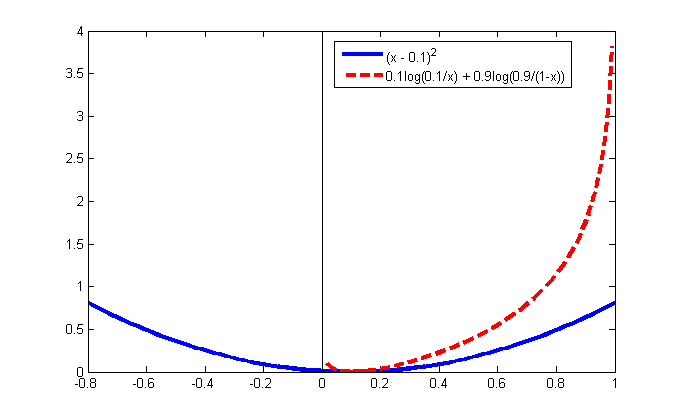
\includegraphics[width=0.75\textwidth]{KLvsSE}
	\caption[So sánh giữa hàm sai biệt KL và hàm lỗi bình phương]{So sánh giữa hàm sai biệt KL và hàm lỗi bình phương với giá trị đầu ra trung bình mong muốn $\rho = 0.1$. Khi giá trị đầu ra trung bình của một nơ-ron ẩn bằng 0, hàm sai biệt KL cho giá trị phạt bằng $\infty$, trong khi đó hàm lỗi bình phương chỉ cho một giá trị phạt rất nhỏ.}
	\label{fig_KLvsSE}
\end{figure}

Mặc dù ``Sparse Coding''sử dụng chuẩn L1 để ràng buộc thưa, nhưng ta thấy rõ ràng là ``Sparse Coding'' sẽ không mắc phải vấn đề nơ-ron ngủ ở trên vì ``Sparse Coding'' không có bộ mã hóa cụ thể như SAEs.
\subsection{Cách Mul-VAE đưa ra gợi ý cho người dùng}
Để khắc phục khó khăn của việc huấn luyện SRAEs với chuẩn L1, chúng tôi đề xuất một phiên bản điều chỉnh của thuật toán ``Stochastic Gradient Descent'' (SGD), gọi là ``Sleep-Wake Stochastic Gradient Descent'' (SW-SGD). Ý tưởng là trong mỗi ``epoch'' của SGD (một ``epoch'' ứng một lần duyệt qua tất cả các mẫu trong tập huấn luyện), ta tính tổng giá trị đầu ra của mỗi nơ-ron ẩn; và sau mỗi ``epoch'', ta kiểm xem có nơ-ron nào ``ngủ'' không (có tổng giá trị đầu ra bằng không) và ``đánh thức'' chúng bằng cách khởi tạo lại véc-tơ trọng số đi vào. Mặc dù cách làm này rất đơn giản, nhưng thí nghiệm của chúng tôi cho thấy nó có thể giúp SRAEs học được thành công các đặc trưng mà không có đặc trưng nào ``ngủ''.

Một cách cụ thể, cho tập huấn luyện không có nhãn $\{x^{(1)}, x^{(2)}, \ldots, x^{(N)}\}$, thuật toán SW-SGD dùng để cực tiểu hóa hàm chi phí sau của SRAEs:
\begin{equation}
\begin{split}
	C(W) &= \frac{1}{N}\sum_{i=1}^N C^{(i)}(W)\\
		 &= \frac{1}{N}\sum_{i=1}^N\left(\|x^{(i)} - \hat{x}^{(i)}\|_2^2 + \lambda \|h^{(i)}\|_1\right)
\end{split}
\end{equation}
Trong đó:
\begin{itemize}
	\item $h^{(i)}$ là véc-tơ đầu ra ở tầng ẩn tương ứng với véc-tơ đầu vào $x^{(i)}$: \[h^{(i)} = \max\left(0, W^{(e)}x^{(i)} + b^{(e)}\right)\]
	\item $\hat{x}^{(i)}$ là véc-tơ tái tạo của véc-tơ đầu vào $x^{(i)}$: \[\hat{x}^{(i)} = W^{(d)}h^{(i)} + b^{(d)}\]
	\item $W=\{W^{(e)}, b^{(e)}, W^{(d)}, b^{(d)}\}$ là các tham số của SRAEs.
\end{itemize}
Từng bước của thuật toán SW-SGD được trình bày ở thuật toán \ref{alg_SW-SGD} (những chỗ thay đổi so với thuật toán SGD ban đầu được \emph{in nghiêng}).
%\begin{leftbar}
%\begin{enumerate}
%	\item Khởi tạo ngẫu nhiên cho $W$.
%	\item Lặp cho đến khi thỏa điều kiện dừng:
%	\begin{itemize}
%		\item \emph{Khởi tạo véc-tơ $s$ gồm có $D_h$ phần tử (với $D_h$ là số lượng nơ-ron ẩn của SRAEs), trong đó mỗi phần tử có giá trị bằng $0$ (phần tử $s_j$ của véc-tơ $s$ dùng để lưu tổng giá trị đầu ra của nơ-ron ẩn $j$ với tất cả các mẫu trong tập huấn luyện sau một ``epoch'').}
%		\item Xáo trộn ngẫu nhiên thứ tự của các mẫu trong tập huấn luyện (thường sẽ giúp hội tụ nhanh hơn).
%		\item Với ``mini-batch'' thứ $b=1,2,\ldots,\frac{N}{B}$ ($N$ là số lượng mẫu trong tập huấn luyện, $B$ là kích thước của ``mini-batch''):
%		\begin{itemize}
%			\item Với mẫu huấn luyện thứ $i=(b-1)B+1, (b-1)B+2, \ldots, bB$:
%			\begin{itemize}
%				\item Lan truyền tiến với véc-tơ đầu vào $x^{(i)}$.
%				\item \emph{Cập nhật véc-tơ $s$: $s = s + h^{(i)}$ (với $h^{(i)}$ là véc-tơ đầu ra ở tầng ẩn tương ứng với véc-tơ đầu vào $x^{(i)}$).}
%				\item Lan truyền ngược và tính véc-tơ đạo hàm riêng $\nabla C^{(i)}(W)$.
%			\end{itemize}
%			\item Cập nhật $W$:
%			\[W = W - \alpha \frac{1}{B} \sum_{i=(b-1)B+1}^{bB} \nabla C^{(i)}(W)\]
%			($\alpha > 0$ là hệ số học)
%		\end{itemize}
%		\item \emph{Kiểm xem có nơ-ron ẩn nào ``ngủ'' (có tổng đầu ra $s_j=0$) và ``đánh thức'' bằng cách khởi tạo lại véc-tơ trọng số đi vào nơ-ron ẩn này.}
%	\end{itemize}
%\end{enumerate}
%\end{leftbar}
\begin{algorithm}
	\newalgname{Thuật toán}
	\caption{Sleep-Wake Stochastic Gradient Descent (SW-SGD)}
	\label{alg_SW-SGD}
	\begin{algorithmic}[1]
		\renewcommand{\algorithmicrequire}{\textbf{Đầu vào:}}
		\renewcommand{\algorithmicensure}{\textbf{Đầu ra:}}
		\algnewcommand\algorithmicoperation{\textbf{Thao tác:}}
		\algnewcommand\Operation{\item[\algorithmicoperation]}
		
		\Require Tập huấn luyện không có nhãn $\{x^{(1)},\ldots,x^{(N)}\}$, hệ số học $\alpha>0$, kích thước ``mini-batch'' B
		\Ensure Bộ tham số $W$ của SRAEs để cho hàm chi phí $C(W)$ đạt cực tiểu
		
		\Operation
		\State Khởi tạo ngẫu nhiên cho $W$
		\While{chưa thỏa điều kiện dừng} \%\% Với mỗi ``epoch''
			\State \parbox[t]{\dimexpr\linewidth-\algorithmicindent}{\emph{Khởi tạo véc-tơ $s$ gồm có $D_h$ phần tử (với $D_h$ là số lượng nơ-ron ẩn của SRAEs), trong đó mỗi phần tử có giá trị bằng $0$ (phần tử $s_j$ của véc-tơ $s$ dùng để lưu tổng giá trị đầu ra của nơ-ron ẩn $j$ với tất cả các mẫu trong tập huấn luyện sau một ``epoch'')}\strut}
			\State \parbox[t]{\dimexpr\linewidth-\algorithmicindent}{Xáo trộn ngẫu nhiên thứ tự của các mẫu trong tập huấn luyện (thường sẽ giúp hội tụ nhanh hơn)\strut}
			\For{b = 1 : N/B} \%\% Với mỗi ``mini-batch''
				\For{i = (b-1)B+1 : bB} \%\% Với mỗi mẫu huấn luyện trong ``mini-batch''
					\State Lan truyền tiến với véc-tơ đầu vào $x^{(i)}$
					\State \parbox[t]{\dimexpr\linewidth-\algorithmicindent}{\emph{Cập nhật véc-tơ $s$: $s = s + h^{(i)}$ \\(với $h^{(i)}$ là véc-tơ đầu ra ở tầng ẩn tương ứng với véc-tơ đầu vào $x^{(i)}$)}\strut}
					\State Lan truyền ngược và tính véc-tơ đạo hàm riêng $\nabla C^{(i)}(W)$
				\EndFor
				\State Cập nhật $W$: $W = W - \alpha \frac{1}{B} \sum_{i=(b-1)B+1}^{bB} \nabla C^{(i)}(W)$ 
			\EndFor
			\State \parbox[t]{\dimexpr\linewidth-\algorithmicindent}{\emph{Kiểm xem có nơ-ron ẩn nào ``ngủ'' (có tổng đầu ra $s_j=0$) và ``đánh thức'' bằng cách khởi tạo lại véc-tơ trọng số đi vào nơ-ron ẩn này}}
		\EndWhile
	\end{algorithmic}
\end{algorithm}

\section{"KL-Annealing"}
Bên cạnh ràng buộc thưa, ràng buộc trọng số cũng là một thành phần quan trọng để làm cho SAEs ``hoạt động''. Tại sao cần phải ràng buộc trọng số? Ví dụ, trong Sparse Coding, ta cần phải ràng buộc các véc-tơ cơ sở được chuẩn hóa (có chiều dài bằng 1); nếu không thì sẽ xảy ra trường hợp là giá trị của hàm chi phí ở công thức (\ref{eq_SparseCoding}) có thể được làm giảm xuống một cách ``tầm thường'' bằng cách chia hệ số cho một số lớn tùy ý và nhân véc-tơ cơ sở tương ứng với cùng số lớn đó (làm như vậy sẽ làm độ thưa giảm xuống tùy ý, còn độ lỗi tái tạo thì giữ nguyên). Các véc-tơ cơ cở trong ``Sparse Coding'' tương ứng với các cột của ma trận trọng số $W^{(d)}$ của bộ giải mã của SAEs (mỗi cột của $W^{(d)}$ ứng với véc-tơ trọng số đi ra tại mỗi nơ-ron ẩn). Như vậy, trong SAEs, ta cũng có thể ràng buộc mỗi cột của $W^{(d)}$ được chuẩn hóa (có chiều dài bằng 1) giống như ở Sparse Coding. Nhưng còn ma trận trọng số $W^{(e)}$ của bộ mã hóa của SAEs? Ta nên ràng buộc $W^{(e)}$ như thế nào cho hợp lý?

Dưới đây là một số cách đã được đề xuất để ràng buộc trọng số của SAEs:
\begin{itemize}
	\item \textbf{Ràng buộc $W^{(d)} = (W^{(e)})^T$}: bộ trọng số được dùng chung cho cả bộ mã hóa và bộ giải mã (cụ thể là $W^{(d)}$ và $W^{(e)}$ là chuyển vị của nhau) \cite{coates2012demystifying}. Cách ràng buộc trọng số này cũng được dùng trong các loại ``Auto-Encoders'' khác như ``Denoising Auto-Encoders'' và ``Contractive Auto-Encoders'' \cite{vincent2008extracting}\cite{rifai2011contractive}\cite{rifai2011HCAEs}. Lưu ý là tất cả \cite{coates2012demystifying}\cite{vincent2008extracting}\cite{rifai2011contractive}\cite{rifai2011HCAEs} đều dùng hàm kích hoạt sigmoid ở tầng ẩn. Trong trường hợp dùng hàm kích hoạt tuyến tính ($f(x) = x$) ở tầng ẩn, ràng buộc $W^{(d)} = (W^{(e)})^T$ sẽ có xu hướng làm cho các véc-tơ cơ sở (các dòng của $W^{(e)}$ hay các cột của $W^{(d)}$) trực giao với nhau và được chuẩn hóa \cite{le2011ica}; nhưng trong trường hợp dùng hàm kích hoạt sigmoid ở tầng ẩn, ta không rõ chuyện gì đang xảy ra. Một điểm lợi của việc dùng chung bộ trọng số là tiết kiệm bộ nhớ lưu trữ; điều này sẽ có ích khi cài đặt song song trên GPU (Graphical Processing Units).
	\item \textbf{Ràng buộc $W^{(d)}$ được chuẩn hóa}: các cột của $W^{(d)}$ được ràng buộc là có độ dài bằng 1 \cite{zeiler2013rectified}. Ràng buộc này tương tự như ở ``Sparse Coding'' và giúp ngăn chặn việc hàm chi phí có thể bị làm giảm xuống một cách ``tầm thường'' như đã nói ở trên. Nhưng còn bộ trọng số $W^{(e)}$ của bộ mã hóa? Chẳng hạn, để công bằng giữa các đặc trưng, ta cũng nên ràng buộc các véc-tơ dòng của $W^{(e)}$ (ứng với các véc-tơ trọng số đi vào các nơ-ron ẩn; các véc-tơ này đóng vai trò như các bộ lọc đặc trưng) có cùng độ dài.
	\item \textbf{Ràng buộc các trọng số có giá trị bình phương nhỏ (weight decay)}: các trọng số của cả bộ mã hóa và bộ giải mã đều được ràng buộc là có độ lớn nhỏ bằng cách phạt tổng bình phương của chúng \cite{goodfellow2009measuring}\cite{coates2011analysis}. Cách ràng buộc này vốn ban đầu được dùng trong mạng nơ-ron học có giám sát để tránh vấn đề quá khớp. Khi áp dụng cho SAEs, ta có hiểu nó là một phiên bản ``mềm'' của cách ràng buộc $W^{(d)}$ được chuẩn hóa ở trên và nhờ đó cũng sẽ giúp cho SAEs tránh khỏi tình trạng hàm chi phí bị giảm xuống một cách ``tầm thường''; ngoài ra, nó còn ràng buộc thêm là các véc-tơ dòng của $W^{(e)}$ (ứng với các bộ lọc đặc trưng) có độ dài xấp xỉ bằng nhau (đều nhỏ). Tuy nhiên, cách ràng buộc này lại làm xuất hiện thêm một siêu tham số; ta không muốn điều này.
\end{itemize}


Với SRAEs (SAEs sử dụng hàm kích hoạt ``rectified linear'' ở tầng ẩn), không rõ là ta nên sử dụng cách ràng buộc trọng số nào trong những cách ở trên. Trong phần này, chúng tôi đề xuất một cách ràng buộc trọng số mới và hợp lý cho SRAEs. Cách ràng buộc này không đưa thêm siêu tham số nào. Cụ thể là, cách ràng buộc trọng số của chúng tôi bao gồm đồng thời hai ràng buộc:
\begin{itemize}
	\item Thứ nhất, chúng tôi ràng buộc ma trận trọng số $W^{(e)}$ của bộ mã hóa và ma trận trọng số $W^{(d)}$ của bộ giải mã là chuyển vị của nhau: $W^{(d)} = (W^{(e)})^T$.
	\item Thứ hai, chúng tôi đồng thời cũng ràng buộc là các véc-tơ dòng của $W^{(e)}$ và các véc-tơ cột của $W^{(d)}$ được chuẩn hóa (có độ dài bằng 1). Ở đây, mỗi véc-tơ dòng của $W^{(e)}$ ứng với véc-tơ trọng số đi vào ở mỗi nơ-ron ẩn, và mỗi véc-tơ cột của $W^{(d)}$ ứng với véc-tơ trọng số đi ra ở mỗi nơ-ron ẩn.
\end{itemize}

Với một véc-tơ đầu vào $x$, nếu ta chỉ chú ý đến các nơ-ron được ``bật'' (có giá trị đầu ra khác không) ở tầng ẩn thì đây là một hệ thống tuyến tính (minh họa ở hình \ref{fig_SRAE}). Do đó, với hai ràng buộc ở trên, SRAEs sẽ chiếu véc-tơ đầu vào $x$ xuống một hệ trục tọa độ cục bộ sao cho từ hệ trục tọa độ này có thể tái tạo được tốt véc-tơ $x$ ban đầu; hệ trục tọa độ cục bộ này bao gồm một số ít các véc-tơ cơ sở (đã được chuẩn hóa) được chọn lựa bởi hàm ``rectified linear'' từ tập lớn các véc-tơ cơ sở. Ta có thể hiểu tập con các véc-tơ cơ sở này biểu diễn vùng không gian PCA cục bộ xung quanh $x$. Như vậy, SRAEs (với ràng buộc trọng số đề xuất của chúng tôi) có thể học được mặt phi tuyến mà ở đó dữ liệu tập trung bằng cách ghép nhiều mặt tuyến tính cục bộ lại với nhau (minh họa ở hình \ref{fig_local_charts}). Mỗi mặt tuyến tính cục bộ được phụ trách bởi một tập con các véc-tơ cơ sở. Điểm lợi ở đây là các véc-tơ cơ sở có thể được dùng chung giữa các mặt tuyến tính cục bộ láng giềng nhau.

\begin{figure}
	\centering
	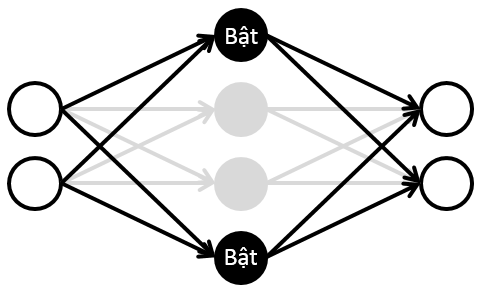
\includegraphics[width=0.6\textwidth]{SRAE}
	\caption[Minh họa SRAEs]{Minh họa SRAEs. Với một véc-tơ đầu vào, nếu ta chỉ chú ý đến các nơ-ron được ``bật'' (có giá trị đầu ra khác không) ở tầng ẩn thì đây là một hệ thống tuyến tính.}
	\label{fig_SRAE}
\end{figure}
\begin{figure}
	\centering
	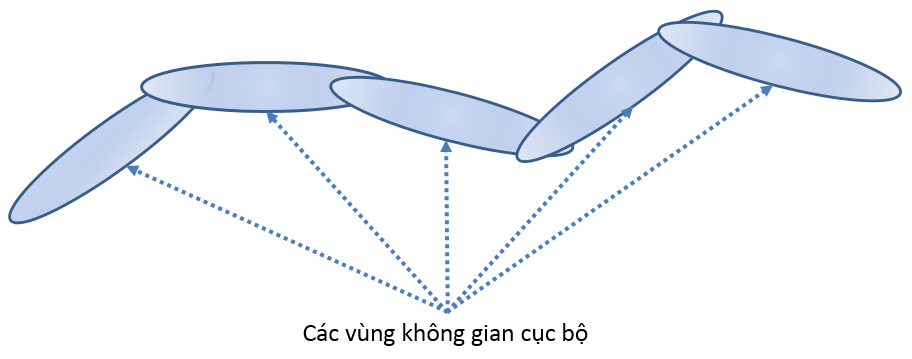
\includegraphics[width=\textwidth]{local_charts}
	\caption[Minh họa mặt phi tuyến mà SRAEs học được]{Với một véc-tơ đầu vào $x$, chỉ có một tập con các nơ-ron ẩn được bật. Tập con các véc-tơ cơ sở tương ứng với tập con các nơ-ron ẩn này biễu diễn một vùng không gian cục bộ xung quanh $x$ (giống như vùng không gian PCA cục bộ). Như vậy, SRAEs (với ràng buộc trọng số đề xuất của chúng tôi) có thể học được mặt phi tuyến mà ở đó dữ liệu tập trung bằng cách ghép nhiều mặt tuyến tính cục bộ lại với nhau. Mỗi mặt tuyến tính cục bộ được phụ trách bởi một tập con các véc-tơ cơ sở. Điểm lợi ở đây là các véc-tơ cơ sở có thể được dùng chung giữa các mặt tuyến tính cục bộ láng giềng nhau.}
	\label{fig_local_charts}
\end{figure}

Như vậy, ta cần phải tối thiểu hóa hàm chi phí của SRAEs với hai ràng buộc trọng số ở trên. Trong khi ràng buộc thứ nhất ($W^{(d)} = (W^{(e)})^T$) có thể được tích hợp dễ dàng vào thuật toán tối ưu hóa ``Stochastic Gradient Descent''  (SGD), ràng buộc thứ hai (các dòng của $W^{(e)}$ và các cột của $W^{(d)}$ được chuẩn hóa) thoạt nhìn khó có thể tích hợp vào thuật toán SGD và có thể ta cần phải sử dụng đến các phương pháp tối ưu hóa phức tạp hơn. Để giải quyết vấn đề này, chúng tôi thay đổi công thức lan truyền tiến của SRAEs như sau:
\begin{equation}
	h = \max(0, \hat{W}^{(e)}x + b^{(e)})
\end{equation}
\begin{equation}
	\hat{x} = (\hat{W}^{(e)})^Th + b^{(d)}
\end{equation}
Trong đó, ma trận $\hat{W}^{(e)}$ là ma trận $W^{(e)}$ với các dòng đã được chuẩn hóa (bằng cách lấy mỗi phần tử trên một dòng của $W^{(e)}$ chia cho căn bậc hai của tổng bình phương của tất cả các phần tử trên dòng đó). Ở đây, các tham số được học vẫn là $W^{(e)}$, $b^{(e)}$, và $b^{(d)}$. Bằng cách này, ta vẫn có thể sử dụng thuật toán SGD như bình thường. Khi đưa thêm bước chuẩn hóa vào công thức lan truyền tiến như vậy, ta cũng cần phải tính lại các đạo hàm riêng của hàm chi phí theo các tham số (sẽ phức tạp hơn so với công thức lan truyền tiến ban đầu). Chúng tôi sử dụng ngôn ngữ lập trình là Theano \cite{bergstra+al:2010-scipy}; nhờ tính năng tính đạo hàm một cách tự động của Theano, ở đây ta sẽ không cần phải tính toán cụ thể công thức của các đạo hàm riêng này.
